\documentclass[phd,tocprelim]{cornell}
%% Added to avoid the \ifpdf name clash error
\let\ifpdf\relax
%
% tocprelim option must be included to put the roman numeral pages in the
% table of contents
%
% The cornellheadings option will make headings completely consistent with
% guidelines.
%
% This sample document was originally provided by Blake Jacquot, and
% fixed up by Andrew Myers.
%
%Some possible packages to include
\usepackage{graphicx,pstricks}
\usepackage{graphics}
\usepackage{moreverb}
\usepackage{subfigure}
\usepackage{epsfig}
\usepackage{subfigure}
\usepackage{hangcaption}
\usepackage{txfonts}
\usepackage{palatino}
\usepackage[LGRx,T1]{fontenc}
\usepackage[utf8]{inputenc}
\usepackage[greek,english]{babel}
\usepackage{hyperref}

\usepackage{textcomp} % defines \textmu, which is now what inputenx seems to use for μ - probably due inpmath.. also \textdegree... but not \textrho
\usepackage{textgreek}

% JaBbA document dependency
\usepackage{enumitem,amssymb}
\usepackage{courier}
\newlist{todolist}{itemize}{2}
\setlist[todolist]{label=$\square$}
\usepackage{pifont}
\usepackage{algorithm}
\usepackage{algpseudocode}
\usepackage{algorithmicx}
\usepackage{amsmath}
\usepackage{mathtools, nccmath}
\usepackage{siunitx}
\DeclarePairedDelimiter\ceil{\lceil}{\rceil}
\DeclarePairedDelimiter\floor{\lfloor}{\rfloor}
\DeclarePairedDelimiter{\nint}\lfloor\rceil
\DeclarePairedDelimiter{\abs}\lvert\rvert
\newcommand{\cmark}{\ding{51}}%
\newcommand{\xmark}{\ding{55}}%
\newcommand{\done}{\rlap{$\square$}{\raisebox{2pt}{\large\hspace{1pt}\cmark}}%
\hspace{-2.5pt}}
\newcommand{\wontfix}{\rlap{$\square$}{\large\hspace{1pt}\xmark}}
% -------
\newcommand{\norm}[1]{\left\lVert#1\right\rVert}
\newcommand{\R}{\mathbb R}
\newcommand{\Q}{\mathbb Q}
\newcommand{\ttt}[1]{\texttt{#1}}
\setlength{\parskip}{0em}
\setlength{\parindent}{1em}


\newtheorem{theorem}{Theorem}[section]
\newtheorem{corollary}{Corollary}[theorem]
\newtheorem{lemma}[theorem]{Lemma}

%if you're having problems with overfull boxes, you may need to increase
%the tolerance to 9999
\tolerance=9999

\bibliographystyle{plain}
%\bibliographystyle{IEEEbib}

\renewcommand{\caption}[1]{\singlespacing\hangcaption{#1}\normalspacing}
\renewcommand{\topfraction}{0.85}
\renewcommand{\textfraction}{0.1}
\renewcommand{\floatpagefraction}{0.75}

%% \title {Structural variations in cancer genomes: representation, inference, and applications}
\title{Illuminating rearranged cancer genome structures through genome graphs}
\author {Xiaotong Yao}
\conferraldate {Aug}{2021}
\degreefield {Ph.D. Computational Biology}
\copyrightholder{Xiaotong Yao}
\copyrightyear{2021}

\begin{document}

\maketitle
\makecopyright

\begin{abstract}
Cancer genomes harbor structural variations (SV), producing various drivers and reflecting . Whole genome sequencing (WGS) characterizes SVs in the form of copy number aberrations (CNA) and junctions. Many simple and complex patterns of SVs have been discovered. Yet, one of the biggest hurdles to analyze SVs is the lack of flexible and general framework to account for the complexity of SVs. SVs inherently alter the coordinate system of the reference genome, thus the interpretation of any junction is dependent on other overlapping junctions. Plus, with short-read WGS, we can only rely on relatively local sequence readouts, making it challenging to reconstruct the long range linear structures of the DNA. To these ends, I present genome graph as a general framework to represent rearranged genomes, which treats genomic sequences as directed graphs, where vertices are single-stranded DNA segments and edges are 3'-5' phosphodiester bonds joining adjacent vertices. Within this framework, I then present a mixed-integer programming algorithm Junction Balance Analysis (JaBbA) to infer integer copy numbers (CN) for vertices and edges from the WGS of a tumor sample. I show that JaBbA not only achieves more accurate CN estimation, more complete genome graphs than other methods, its robust recapitulation of junction copy numbers (JCN) serves a pivotal role in discovering distinct patterns of complex rearrangements from large-scale pan-cancer WGS studies. Finally, to investigate the SV outcomes of natural telomere crisis, an inevitable obstacle most cancer must overcome and has been linked to complex SV patterns, I use the genome graph framework to reconstruct the SV events in lineages of human fibroblast cells surviving natural telomere crisis by induced telomerase expression. To sum up, genome graph with the Junction Balance Analysis algorithm enable a general, robust analysis framework that help elucidate the complexity of SVs in cancer genome.
\end{abstract}

\begin{biosketch}
Xiaotong Yao has had strong interest in biology from an early age and later developed an appreciation for using computational methods to answer biological questions. His interest for computational biology started with systems biology and synthetic biology by participating in the 2011 International Genetically Engineered Machine Competition. Subsequently, he curated lipid metabolic pathways in the \textit{Streptomyces avermitilis} metabolic network. To get formally trained in computational biology, he joined the Master's program in Bioinformatics and Systems Biology at the Biology Department of New York University, where he built predictive models for protein sumoylation from public protein function databases. Following a passion for precision medicine, in 2015, he became a PhD student in the Tri-institute Program in Computational Biology and Medicine at Weill Cornell Medicine, focusing on cancer genomics, and in 2016 he joined Dr. Marcin Imielinski's lab to persue his dissertation research in using genome graphs to model complex structural variations in cancer whole genomes.
\end{biosketch}

\begin{dedication}
To Rosalind Yao and Shan Huang.
\end{dedication}

\begin{acknowledgements}
Marcin
Kevin
Julie
Aditya
Committee
Collaborators
Program
Sample donors
\end{acknowledgements}

\contentspage
\tablelistpage
\figurelistpage
\abbrlist

SV -- structural variation

WGS -- whole genome sequencing

CN -- copy number

CNA -- copy number aberration

JaBbA -- Junction Balance Analysis

\symlist

\normalspacing \setcounter{page}{1} \pagenumbering{arabic}
\pagestyle{cornell} \addtolength{\parskip}{0.5\baselineskip}

%%%%%%%%%%%%%%%%%%%%%%%%%%%%%%%%%%%%%%%%%%%%%%%
%% Chapter 1: introduction
%%%%%%%%%%%%%%%%%%%%%%%%%%%%%%%%%%%%%%%%%%%%%%%
%% To motivate what comes next.
\chapter{Introduction}

\section{Complexity of SVs in the cancer genomes}
Genomic instability is a hallmark of cancer and the complete pool of genomic variants in cancer are shaped by various mutagenesis pathways and somatic evolution. With whole genome sequencing (WGS), we are profiling large numbers of cancer genomes revealing ubiquitous yet heterogeneous patterns of single nucleotide variations (SNV), insertions and deletions (INDEL), and structural variations (SV). However, the discoveries of SNV and INDEL patterns have been outpacing that of SVs, exemplified by the distillation of mutation signatures from large-scale mutation profiles described in local sequence context of the substitution. Even though we have known for a long time that cancer genomes present widespread aneuploidy and rearrangements, it still remains challenging to characterize the full spectrum of SVs in cancer.

There are many reasons to this, but a fundamental one is that the SVs in cancer genomes are complex and there lacks a suitable framework to account for it. Practically, SVs are detected in two ways, the discordant read pairing or sequences indicate a variant junction -- two disconnected genomic loci in reference genome that are adjacent in the sample; and the deviated read depth mapped to a genomic interval reflect aberrant copy numbers. By combining these two facets of the rearranged genome, various cancer WGS studies have inferred a plethora of complex SV patterns. A prominent example is chromothripsis, theorized to originate from shattering a chromosome arm into pieces and erroroneously rejoined a subset of them in random order. Such processes can generate up to hundreds of junctions at random locations and with random orientations, while leaving an oscillating CN profile due to loss of interspersed. Recent pan-cancer whole genome analyses estimated chromothripsis-like events exist in as many as xx\% of pan-cancer genomes (cite PCAWG SV and Park).

Despite these observations, most studies on genomic structural variations have been geared towards germline genomes, whose SVs are dominated by simple SV classes, namely tandem duplications, simple deletions, and inversions. Although more complex patterns have also been characterized, they are (expectedly) rare relative to the simpler ones. Since each simple SV only contains one (tandem duplications and deletions) or two junctions (inversions and balanced translocations), it is usually convenient to apply the substitution model that has long been the standard practice in representing and storing small genomic variants, such that one variant is represented as an edit of a fixed location of the reference genome and in most cases each variant can be interepreted independently from the other variants.

The limitation of this approach is visible even in the simplest form of complex SV. Considering the toy model in (Fig 1A, adapted from MI/JM's review), where a unrearranged genomic contig \textit{ABCDE} underwent two rounds of tandem duplications, yet when mapped to the reference genome, the second junction appeared to be consistent with a deletion. As a result, the development of a more general framework to analyze complex SVs is needed.

\section{Representation of structural variations with genome graphs}
Graphs have been widely used to model genomic sequences for decades, with \textit{de novo} assembly as one of the fields most heavily reliant (citation SGA, Fermi, etc.). One way to describe sequence as graphs is that each vertex is the sequence of a contiguous DNA segment (contig) and following the adjacencies among vertices one can thread a path (or cycle) to obtain longer sequence and eventually approach a genome. In resequencing studies, we map reads to locations in an existing reference genome, and identify variants based on the discrepancy between reads and the mapped reference sequence. Nevertheless, we can apply a similar idea of modeling, now replacing actual DNA sequences to the genomic intervals they map to in the reference. There have been several studies employed the concept of \textit{interval graph} to model the somatic SVs in cancer genomes. which treats xxx (describe the interval graph models). %% TODO

In our published works and this dissertation, we have formulated a directed skew-symmetric graph data structure, called \textit{genome graph}, that is dual to the variations of interval graphs decribed above. Like the previous work, we will show that genome graphs can represent genomic rearrangements based on a reference genome and serve as a scaffold to inferring 

\section{Reconstruction of junction-balanced genome graphs}
While conceptually interval graph has been an advancement over the overly-simplistic substitution model, the cancer genomics research community has not fully adopted it as the mainstream framework for SV analysis. The main reason is that the numeric quality of the copy numbers in the reconstructed graphs have not shown high enough fidelity for the heterogeneous lanscape of complex somatic SVs, as well as varying sample purity. There have been several approaches proposed with slightly different objectives, nevertheless share the common theme of fitting CN to the DNA segments while deciding the subset of junctions to include.

\section{From patterns to mechanisms to etiology}
The ultimate goal of studying patterns of SVs is to find common classes out of large panels of tumors, and link them back to the possible mechanisms from which specific SVs arise. For example, telomere crisis.

Early efforts in this realm successfully identified many distinct patterns.

\section{Evolution of SVs after telomere crisis}

%%%%%%%%%%%%%%%%%%%%%%%%%%%%%%%%%%%%%%%%%%%%%%%
%% Chapter 2: formalize genome graphs and JaBbA
%%%%%%%%%%%%%%%%%%%%%%%%%%%%%%%%%%%%%%%%%%%%%%%
\chapter{Junction-balanced genome graphs represent structurally altered genomes}
In this chapter, I give formal definitions of a genome graph, a junction balanced genome graph, and Junction Balance Analysis to infer integer copy numbers from short-read whole genome sequencing data. I also establish the correspondance between a walk on a genome graph to the underlying karyotype and show genome graphs can unify a diverse array of putative functional events including fusion genes and enhancer hijiacking. Last but not least, taking advantage of our novel interactive genome browser \textit{gGnome.js}, I show that our complete toolset can serve as an intuitive portal for oncologists to fully take advantage of cancer WGS data.

\section{Genome graph as a general data structure to represent rearranged genome}
We start by formally defining a reference genome, a genome graph, a junction.

\subsection{Reference genome}
Let the reference genome $\mathcal{C}$ comprise $c$ pairs of strings, labeled $C^i$ and $C^{-i}, i \in 1,\dots,c$. Each string pair $\{C^i, C^{-i}\}, i \in 1,\dots, c$ is called a \textit{chromosome}, and each string in that pair is called a \textit{strand}. We use $C^i$ and $C^{-i}$ to refer to "positive" and "negative" strands of chromosome $i$, each having length $L_i \in \mathbb{N}$. We use brackets to denote substrings on these strands. For example, $C^{i}[q,r]$ refers to the substring of $C^{i}$ beginning at position $q$ and ending at position $r$ (inclusive) where $q \le r \in 1,\dots,L_i$. We also use $C^{i}_q$ as a shorthand for $C^{i}[q,q]$. In the remainder of this dissertation, we call $C^{i}[q,r], i \in 1, \dots, c, q \le r \in 1, \dots, L_i$ a signed \textit{genomic interval}. 

Every signed genomic interval has a "reverse complement" $C^{-i}[q,r]$ and together they make a double stranded ("unsigned") interval $C^{\pm{i}[q,r]}$. As is the convention in defining reference genomes, on the positive strand $C^i$, the coordinate increases from 5' end to 3' end. In other words, $C^{i}_q$ is the 5' end of $C^{i}[q,r]$, and $C^{i}_r$ its 3' end. Two intervals $C^{i}[q_1, r_1], C^{j}[q_2, r_2]$ are said to overlap if $i = j$ and either $q_2 \le r_1$ or $q_1 \le r_2$.

\subsection{Genome graph}
% definition in as plain language as possible
% need to define: reference genome, interval, signed interval, junction
Based on a reference genome $C$, we define genome graph $G = (V, E)$, where the vertices $V$ is a multi-set of signed intervals, and edges $E$ is a set of directed adjacencies representing the 3'-5' phosphodiester bonds between vertices. Since genomic DNA is a pair of reverse complement strands, we restrict $G$ to be skew-symmetric (see formal definitions in Methods) with the mapping function $r$ "reverse complement"  \cite{Goldberg1996-qm}, such that for any vertex $v \in V$, there exists its \textit{symmetric} vertex $\bar{v} = r(v) \in V$, and for any edge $e = (v_1, v_2) \in E$, $\bar{e} = r(e) = (\bar{v_2}, \bar{v_1}) \in E$. Intuitively, each reverse complement pair of vertices represent a double stranded DNA segment within the reference genome. Since any vertex maps to a genomic interval, we denote its location in the reference genome with $C^{i}[q,r]$.

To denote the location of edges, suppose we have an edge $e = (v_1, v_2), v_1$

Subsequently, there are two types of edges. \textit{REF} edges are the ones that are connecting vertices adjacent in the reference genome, and \textit{ALT} are neo-adjacencies that are not present in the reference genome resulting from rearrangements (Fig2). A reverse complement pair of vertices $\{v, \bar{v}\}$ compose a double-stranded DNA segment (segment for short); a reverse complement pair of edges $\{e, \bar{e}\}$ compose a junction. Analogous to an assembly graph, to produce a substring in the genome, is equivalent to traveling through a walk $w = (v_1, e_1, v_2, e_2, \dots, e_k, v_k)$, where each edge $e_i = (v_i, v_{i+1}), i \in 1, 2, \dots, k-1$, at the same time its reverse complement walk $\bar{w} = (\bar{v_k}, \bar{e_k}, \bar{v_{k-1}}, \dots, \bar{e_1}, \bar{v_1})$.


\subsection{Breakends and junctions}
%% is this a legit syntax for ordered set? "()"?
To describe a rearranged and copy number altered reference genome, we partition $\mathcal{C}$ according to a collection of \textit{breakends} $\mathcal{B}$. We also define a set of \textit{junctions} $\mathcal{A}$ representing alternative adjacencies between a set of the  breakends in $\mathcal{B}$. Each $B^i \in \mathcal{B},\ i \in 1,\ldots,c$ is an ordered and unique sequence of integer coordinates $B^i = (B^i_k), 1 \le B^i_k \le L_i$ on chromosome $i$, where $B^i_1$ = 1 and $B^i_{|B^i|} = L^i$.  Each junction $A \in \mathcal{A}$ is a tuple $(i_1,r_1,i_2,r_2),\ r_1 \in B^{|i_1|}, r_2 \in B^{|i_2|}$, $|i_1|, |i_2| \in  1, \ldots, c$ representing a (3'-5' phosphodiester) bond between the position $r_1 + \frac{-sgn(i_1)+1}{2}$ on chromosome / strand $C^{i_1}$ and position $r_2+\frac{sgn(i_2)+1}{2}$ on chromosome / strand $C^{i_2}$.  For every adjacency $A = (i_1,r_1,i_2,r_2) \in \mathcal{A}$ we require $\mathcal{A}$ to contain the reverse complement adjacency $\bar{A} = (-i_2,r_2, -i_1,r_1)$. The adjacencies in $\mathcal{A}$ are "alternative" relative to a set of "reference adjacencies" $\mathcal{R}$ implied by $B^i$, comprising tuples $(i, B^i_k, i, B^i_k)$ and $(-i, B^i_k, -i, B^i_k)$ for each breakend $B^i_k, k\in 1,\dots,|B^i|$ in each chromosome $i \in 1,\ldots,c$.

\subsection{Junction-balanced genome graph}
We define a mapping $\kappa:\{V_I \cup E\}\rightarrow \mathbb{N}$ of non-negative integer copy number (CN) to vertices and edges of $G$, where $\kappa(v),v \in V_I$ and  $\kappa(e),e \in E$ represent the CN of vertex $v$ and edge $e$, respectively.  The principle of \textit{junction balance} constrains the CN of every vertex to be equal to the sum of its incoming edges and the sum of its outgoing edges.  Formally, the junction balance constraint is stated as follows:

\begin{equation}
    \label{eq:junction_balance_constraint}
\kappa(v)= \sum_{e\in E^-(v)} \kappa(e) = \sum_{e\in E^+(v)} \kappa(e)
\end{equation}

In addition we require the CN $\kappa$ to obey \textit{skew-symmetry}, which means that every vertex must have the same copy number as its RC.

\begin{equation}
    \label{eq:skew_symmetry}
\kappa(v) = \kappa(\bar{v}),\ \forall_{v \in V} \quad \kappa(e) = \kappa(\bar{e}),\ \forall_{e \in E} 
\end{equation}

We call the combination $(G,\kappa)$ for which $\kappa$ satisfies Eqs. \ref{eq:junction_balance_constraint}-\ref{eq:skew_symmetry} a \textit{junction-balanced genome graph} (JBGG).

% 
Following the above definitions, except for whole genome/chromosome/contig gain or losses or foreign sequence insertions, every structural change of a genome can be effectively seen as generating new adjacencies (ALT edges) between previously non-adjacent vertices.

% Note that this abstraction does not make assumptions about the mechanism by which the new adjacencies arise, rather it describes the difference of states after an SV event.

Extending the properties of $r$ to any function of vertices or edges, we call a function $f(v), v \in V(G)$ or $f(e), e \in E(G)$ as skew-symmetric if $f(v) = f(\bar{v})$, $f(e)=f(\bar{e})$. One such function is copy number $\kappa : G \rightarrow \mathbb{N}$, as for double stranded DNA the copy number of one strand should always be equal to its reverse complement.

Intuitively, a walk along on a genome graph maps to a DNA sequence and a genome graph is a compilation of all possible linear sequences that could result from rearranging the reference genome assuming the junctions are completely known. This idea is similar to the assembly graph in \textit{de novo} assembly, except we are pre-defined within a linear reference genome and adding further rearrangements.

\section{Implementation of genome graphs in gGnome package}
% noteworthy implementation details
We 

% construction
In the most basic form, a genome graph can be initiated with a reference genome alone, where each node is a chromosome and no edges exist (\texttt{gG()}). On top of that, we can segment the whole genome based on a set of breakpoint coordinates, by automatically connecting two consecutive nodes with a (pair of reverse complement) REF edge (\texttt{gG(breaks = breakpoints)}). When a ALT junction emerges, it joins two breakends that are not adjacent in reference genome to form new (pair of reverse complement) ALT edges (\texttt{gG(juncs = junctions)}).

More often in practical scenarios, we start from a copy number-annotated genome graph inferred from WGS. gGnome allows one to parse the results from most of the existing genome graph reconstruction methods (JaBbA, ReMixT, Weaver, PREGO, RCK, CouGaR, AmpliconArchitect). 

% subgraph
With a genome graph, we can make a series of queries based on vertex and edge metadata.

\section{Neo-connectivities on a genome graph encode putative functional events}

As explained in the previous sections, a walk (and its reverse complement walk) on a genome graph maps to a linear DNA sequence. If there exists a possible walk between two vertices it means the genomic elements within the two vertices may be connected on a contiguous DNA segment in the sample, if and only if all the ALT edges along the walk are phased in cis. A pair of ALT edges phased in cis means there are at least one copy of them found on the same DNA molecule; while none such copy is found they are deemed phased in trans. In reality, due to the large size of the genome and the limited read-length or effective range (e.g. for linked reads), complete phasing of all junctions is near impossible for most cases. However, the connectivities between genomic regions on the un-phased or partially phased genome graphs can serve as an approximation. 

As we established in earlier sections, a complete genome graph should enclose all the walks corresponding to the studied genome, so if any copy of two genomic loci are on the same part of a DNA molecule, that segment should have a corresponding walk on the complete genome graph. Based on this observation, the new genomic distance after rearrangements between any copy of two loci is summing over the width of vertices plus the within-vertex distances to the incident ends along the walk for the starting and terminating vertices. Thus, even when it is not possible to exactly decompress the graph to the walks consistent with the actual karyotypes, we know that the real shortest genomic distance between any copy of two loci should not be shorter than the shortest path distance on the complete genome graph.

Admittedly, there may never be a complete genome graph constructed with the current technologies, and it is always possible that we failed to identify certain junction that cut some genomic distances even shorter. Nevertheless, as shown in (Behr 2021, BioRxiv), the state of the art short-read WGS should be effective at catching the majority of somatic rearrangements. Plus, even with the imperfect genome graphs, we can already expand the repertoire of functional genomic events. We use this approximation to show that potential functional events of arbitrary complexity can be represented as walks on genome graphs, exemplified by bridged fusion genes and enhancer hijacking. To do that, I reconstructed JBGG from PCAWG consensus somatic junctions and copy numbers with the function \textit{balance} in the gGnome package.

Some fusion genes have long been established as cancer drivers (citation) and even successful drug targets (citation); some have also been shown to encode chimeric proteins that can trigger immune responses as neoantigens (citation). Expectedly, most fusion genes found to date are created by one somatic junction, as it requires fewer junctions to create and has simpler topology to detect. However, in theory, there should be no biological restraint against a more complex, multi-junction fusion gene. Indeed, recent large pan-cancer whole genome and transcriptome profiling efforts have identified numerous such examples termed bridged fusions (citation PCAWG). Naturally following our above definition, any fusion genes, no matter how many somatic junctions is involved, can be represented as a walk $w = (v_1, e_1, v_2, ..., e_{k-1}, v_k)$ on the corresponding genome graph, where the 5’ partner is at the outgoing end of $v_1$ and the 3’ partner is at the receiving end of $v_k$ (Fig x). Here I show an example walk of xxx—xxx fusion found by the PCAWG Transcriptome working group (citation) along with the supporting reads from the RNA-seq. By our graph-based SV event classification, this junction was part of a large scale xx (described in the next chapter).


\section{Junction Balance Analysis infers copy numbers on genome graphs from whole genome sequencing}


\subsection{Formulation of the mixed-integer quadratic programming problem}

\begin{figure*}[!t]
    \centering
    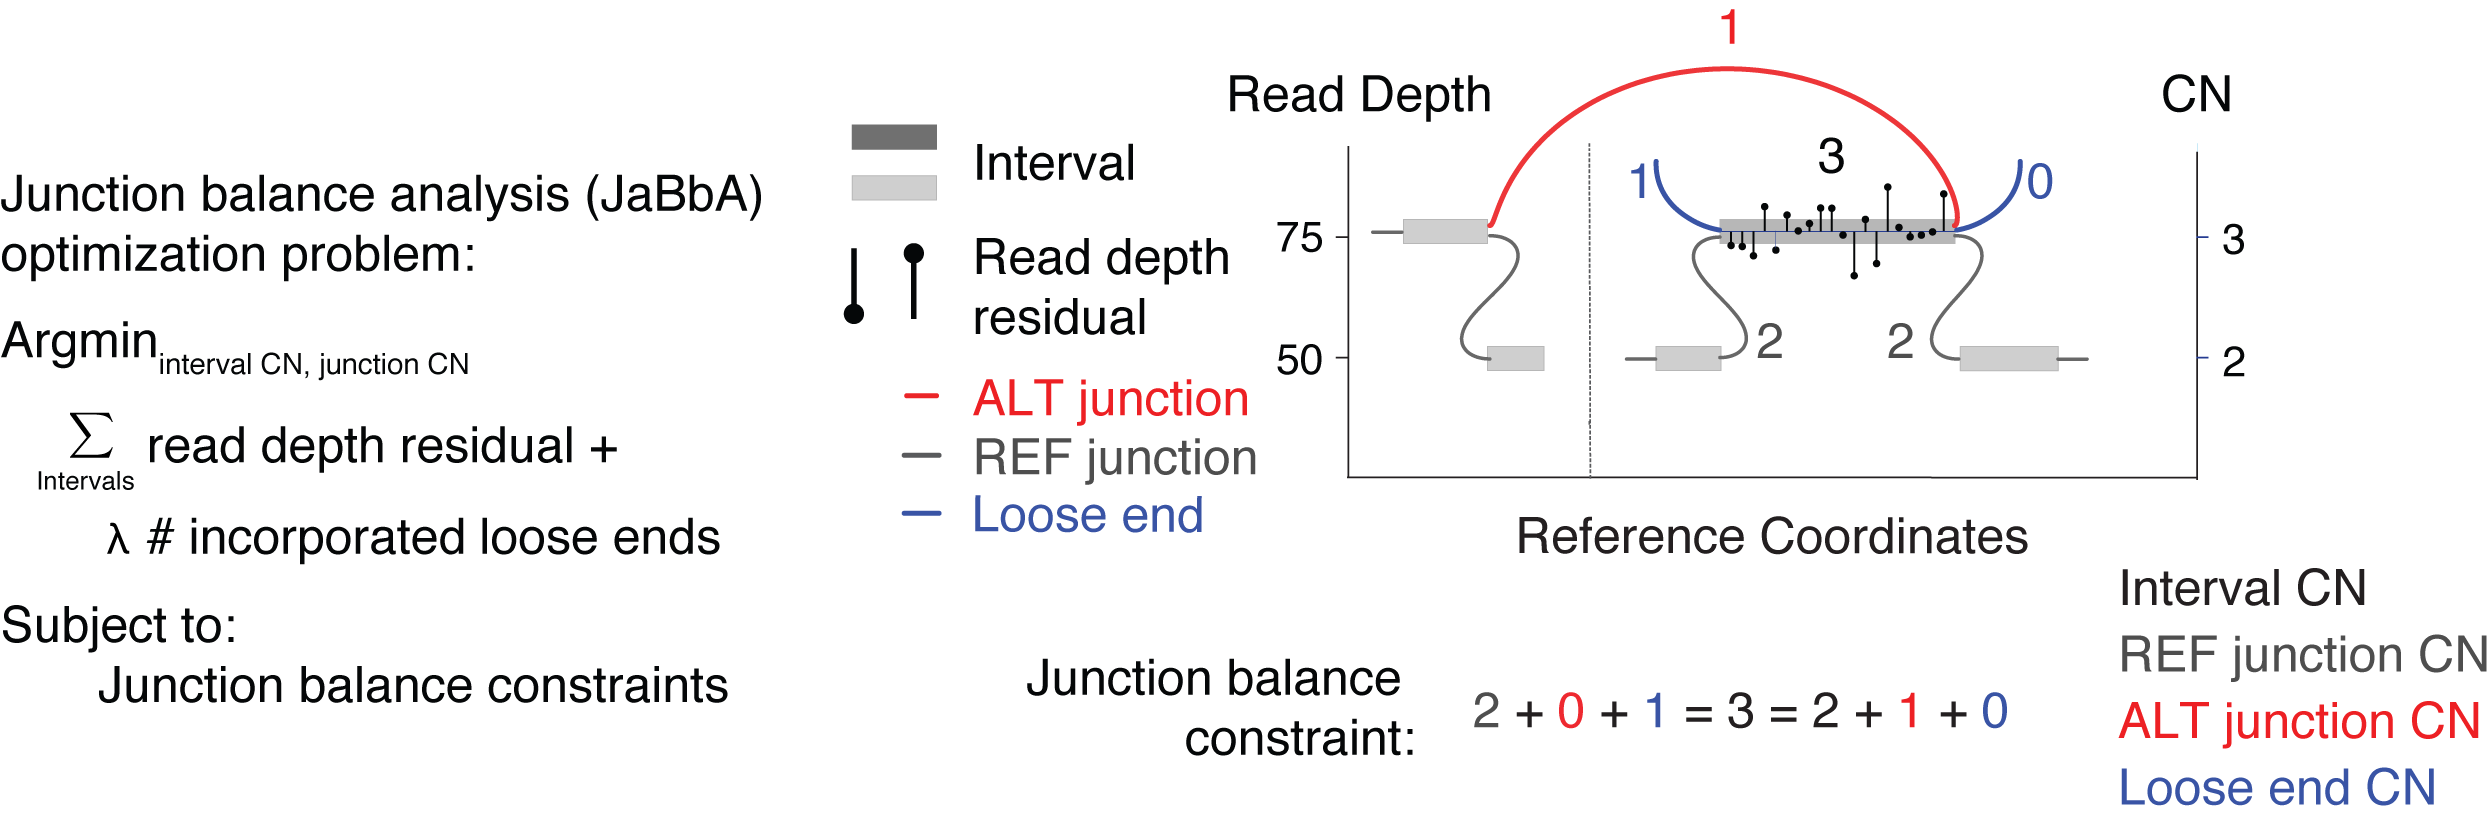
\includegraphics[width=0.95\linewidth]{figures/600ppi/jabba_formulation.png}
    \caption{\textbf{Formulation of Junction Balance Analysis} xxxx...}
    \label{fig:jabba_formulation}
\end{figure*}

We developed an algorithm, JaBbA, to infer junction-balanced genome graphs with high fidelity. Analogous to previous approaches, we define a (directed) genome graph of vertices representing strands of genomic segments and edges  representing a pair of 3' and 5' DNA ends that are adjacent in the reference genome (REF edge) or connected through rearrangement (ALT edge). A \textit{junction balanced genome-graph} assigns every vertex and edge in the graph an integer CN, while enforcing the constraint that the dosage of every interval (vertex) is equal to the sum of the JCN of the incoming (or similarly, outgoing) junctions (\textbf{Fig. \ref{fig:jabba_formulation}}).  The MIP optimization solved by JaBbA minimizes the residual between observed read depth and inferred interval dosage through joint assignment of CN to intervals and junctions (\textbf{Fig. {fig:Fig1}B, Fig. {fig:S1}C}, sec:methods).

\subsection{JaBbA pipeline}
Junction Balance Analysis (JaBbA, \url{https://github.com/mskilab/JaBbA}) is an R package freely available under the MIT license. The required inputs to JaBbA are binned (e.g. 200bp) and normalized read depth data $y$, purity $\alpha$, ploidy $\tau$, a set of junctions $\mathcal{A}$ (see mathematical formulation above), and a hyperparameter $\lambda$. The key output is a \texttt{gGraph} object representing a junction-balanced genome graph (i.e. solution to \textbf{Eq. \ref{eq:MIQP}}) which can be queried and analyzed using downstream algorithms, e.g. SV event classification algorithms in the \texttt{gGnome} package (\url{https://github.com/mskilab/gGnome}, see "Structural variant event classification" section below). The workflow of JaBbA is composed of four phases: read depth preprocessing, graph building, JaBbA model fitting, and postprocessing.

\subsubsection*{Data preprocessing}

\subsubsection*{Graph partitioning}

% \section{Automatic tuning of convergence criteria to improve the performance of harder problems}

\subsubsection*{Post processing and allelic CN fitting}

\section{JaBbA robustly produce accurate copy numbers for DNA segments and junctions}
JaBbA differs primarily from previous genome graph methods in its robust modeling of WGS read depth noise and explicit accounting of false negative junctions, also called loose ends (see \nameref{sec:methods}). In our benchmarking experiments, JaBbA inferred JCN with consistently higher fidelity than published genome graph-based methods (ReMixT \cite{McPherson2017-ry}, Weaver \cite{Li2016-qa}, PREGO \cite{Oesper2012-vw}) across a wide range of tumor purities (\textbf{Fig. \ref{fig:S1}D-E}). In addition, JaBbA qualitatively outperformed genome graph-based methods and even classic (i.e. non-graph based) CNA callers (BIC-seq \cite{Xi2011-oa} and CONSERTING \cite{Chen2015-sw}) in estimating interval CN and change point locations across a wide range of tumor purities (\textbf{Fig. \ref{fig:S1}F-I}). These results show that JaBbA is the first genome graph SV caller to accurately infer the topology of JCN while approaching (or exceeding) the fidelity of classic CNA callers. 

We also validated JaBbA's estimates of JCN from short-read WGS with 10X Chromium linked-read WGS, which provides a more direct readout of JCN with its high number of long junction-spanning fragments. In the breast cancer cell line HCC1954, JaBbA-derived JCN estimates closely correlated with the coverage of junction-spanning linked-read barcodes ($R^2 = 0.91$, \textbf{Fig. \ref{fig:Fig1}C}). This included examples of low JCN (e.g. JCN = 1) junctions connecting both low and high CN intervals, as well as high JCN (JCN = 10)  junctions (\textbf{Fig. \ref{fig:Fig1}D}). These results show that JCN is a property that can be robustly inferred from short-read WGS and is independent from (interval) CN. 

\section{Interactive visualization of genome graphs in arbitrary genomic windows}


\section{Discussion}

%%%%%%%%%%%%%%%%%%%%%%%%%%%%%%%%%%%%%%%%%%%%%%%
%% Chapter 3: discovery of novel SV patterns
%%%%%%%%%%%%%%%%%%%%%%%%%%%%%%%%%%%%%%%%%%%%%%%
\chapter{Distinct Classes of Complex Structural Variation Uncovered across Thousands of Cancer Genome Graphs}
In this chapter I will describe the discovery of three distinct types of complex SV events from 2778 genome graphs built with JaBbA from a pan-cancer cohort of over 30 types of cancers. Furthermore, I will show that the patients in this cohort can be stratified based on 13 simple to complex rearrangement patterns to clusters of differential overall survival, tumor type enrichment, and association with specific germline or somatic alterations.

\section{Analysis of pan-cancer genome graphs}
To investigate the topology of JCN across cancers, we assembled a dataset comprising 2,813 short-read WGS tumor or cell line samples spanning 31 primary tumor types (Table \ref{tab:S1}), including WGS for 539 previously unpublished cases  (\textbf{Table \ref{tab:S2}}). In total, our analysis included 1,648 WGS samples not included in the Pan-Cancer Analysis of Whole Genomes (PCAWG) effort \cite{pcawg_marker2020-yi}.  Application of harmonized pipelines followed by JaBbA (\textbf{Fig. \ref{fig:Fig1}B}) yielded 2,778 high quality genome graphs (\textbf{Fig. \ref{fig:Fig1}E}, see \nameref{sec:methods} for sample characteristics and exclusion criteria). 

% TODO: fix the table insertion
% \begin{table}[!ht]
%     \captionsetup{justification=raggedright,singlelinecheck=off}
%     \caption{\textbf{Pan-cancer WGS cohort summary, related to Figure \ref{fig:Fig1}} Summary (table in pdf format) of the number of samples from each tumor type and the number of cell line samples of a tumor type.}
%     \label{tab:S1}
% \end{table}

% \begin{table}[!ht]
%     \captionsetup{justification=raggedright,singlelinecheck=off}
%     \caption{\textbf{Sources of pan-cancer WGS datasets used in this study, related to Figure \ref{fig:Fig1}} Summary (table in pdf format) of the number of samples from each dataset, the completeness of the pipelines, and the citation if the dataset is published before.}
%     \label{tab:S2}
% \end{table}

Analyzing junction-balanced genome graph topology, we identified subgraphs associated with previously identified complex rearrangement patterns such as chromothripsis, chromoplexy, and TICs (\textbf{Fig. \ref{fig:Fig1}B, right panel}) implementing criteria described in previous publications within our framework (see \nameref{sec:methods}). Consistent with our 10X Chromium WGS benchmarks (see above) (\textbf{Fig. \ref{fig:Fig1}C}), we observed wide variation in inferred JCN across our datasets which correlated with observed read depth changes at breakends (\textbf{Fig. \ref{fig:Fig1}F}). While the vast majority of junctions demonstrated low-JCN (JCN $\leq$ 3), we observed a long tail of junctions with elevated– (JCN > 3) and high-JCN (JCN > 7) (\textbf{Fig. \ref{fig:Fig1}G}).

\section{Low JCN clusters of deletion-like and duplication-like junctions form rigma and pyrgo}
To distinguish between complex SV patterns associated with low-JCN vs. high-JCN junctions, we identified junction clusters based on their overlapping footprints on the reference and labeled each cluster as high- / low- JCN on the basis of its highest copy junction (high-JCN thresholded at $>$ 7). Considering clusters harboring three or more junctions, we found low-JCN clusters were significantly more likely to be dominated ($>$ 90\% representation of that type) by DEL-like ($P < \SI{2.2e-16}{}$, z-test, logistic regression) or DUP-like junctions ($P < \SI{2.2e-16}{}$) (\textbf{Fig. \ref{fig:S2}A}).

To rigorously nominate clusters of low copy DUP-like and DEL-like junctions within each tumor sample, we identified genomic tiles (1 Mbp width, 500 kbp stride) enriched in low-JCN of a given type (e.g. DEL-like) relative to a calibrated gamma-Poisson background model (see \nameref{sec:methods}). In each analysis, non-outlier tiles harbored apparent simple deletions or duplications (\textbf{Fig. \ref{fig:Fig2}A-B}). In contrast, outlier bins in the DUP-like model resembled "towers" of low-JCN DUP-like junctions  (\textbf{Fig. \ref{fig:Fig2}A, top right}) that we named \textit{pyrgo} (\textgreek{p'urgos}, Greek meaning tower). Outlier loci in the DEL-like models comprised subgraphs of interval CN "chasms" flanked by low-JCN DEL-like junctions whose interval CN often reached 0 (\textbf{Fig. \ref{fig:Fig2}B, top left}).  We named these patterns \textit{rigma} (ρήγμα, Greek meaning rift).

\section{Tyfonas is massively rearranged amplicon associated with elevated number of fusion genes}
We then sought to investigate the rearrangement patterns associated with high-JCN junctions (JCN $>$ 7) in our genome graphs.  \textit{A priori}, a junction at such an extreme of JCN may evolve through a double minute, BFBC, or an as yet undescribed mechanism for duplicating already rearranged DNA. To characterize classes of  amplification events associated with these high-JCN junctions, we first identified 12,588 subgraphs harboring an interval CN of at least twice ploidy among the 2,487 unique genome graphs (by patient) (\textbf{Fig. \ref{fig:Figure4}A}), then identified among these amplicons (amplified clusters within a genome) those that harbor at least one junction with JCN $>$ 7.  We annotated the resulting 1,703 high-JCN amplicons according to several features: 1) the maximum JCN normalized by the maximal interval CN, 2) the summed JCN associated with fold back inversion junctions (INV-like junctions that terminate and begin at nearly the same location in the genome) relative to the maximal interval CN, and 3) the number of junctions with elevated JCN (JCN>3) (see \nameref{sec:methods}).

Clustering and classification of amplicons (\textbf{Fig. \ref{fig:Figure4}B}) on the basis of these three features yielded three stable clusters (\textbf{Fig. \ref{fig:S4}A-B}) (see \nameref{sec:methods}).  Upon visual inspection, the first group, harboring low fold-back JCN but high maximal JCN, contained amplicons comprising a single high-JCN junction forming a high CN circular path in the graph (\textbf{Fig. \ref{fig:Figure4}C}) as well as more complex cyclic patterns spanning multiple discontiguous loci, consistent with a double minute.  The second group, demonstrating high fold-back JCN ($>$ 0.5), a low burden of elevated-JCN junctions ($<$ 26), and a "stair step" pattern of copy gains, was consistent with a BFBC (\textbf{Fig. \ref{fig:Figure4}D}) \cite{Zakov:2013cm}. The third group contained both high fold-back JCN ($\geq$0.50) and a significant burden of elevated JCN junctions ($\geq$26).  Upon visual inspection, these amplicons comprised dense webs of elevated  JCN junctions across subgraphs compris $>$ 100 Mbp of genomic material and often reaching CNs higher than 50 (\textbf{Fig. \ref{fig:S4}C}).  We dubbed these extremely large amplicons, which did not fit in previously defined categories, \textit{tyfonas} (τύφωνας, Greek meaning typhoon) (\textbf{Fig. \ref{fig:Figure4}E}).

\section{Clusters of pan-cancer patients based on SV event burdens show differential prognosis and is associated with tumor types and genetic backgrounds}
Tallying normalized junction counts across 13 event categories and 2,487 patients, we found 14 stable clusters using standard model selection metrics (\textbf{Fig. \ref{fig:Fig_cluster}A, Fig. \ref{fig:S7}A-B, Table \ref{tab:S3}}). Most clusters were dominated by 1-3 event types (e.g. CT = chromothripsis, BR = BFBC, rigma, DDT = deletion, duplication, TIC) with the exception of two: QUIET (few events) and SPRS (sparse, miscellaneous events).

Consistent with previous reports, the CT cluster was significantly enriched in prostate adenocarcinoma  (PRAD, $P = \SI{2.05e-5}{}$, $OR = 1.99$, single-sided z-test, Bayesian logistic regression, \cite{Kovtun2015-kq}) and glioblastoma multiforme (GBM, $P = \SI{5.00e-8}{}$, $OR = 2.61$, \cite{Furgason2015-rv})  (\textbf{Fig. \ref{fig:Fig_cluster}B}). Similarly, the CP (chromoplexy) cluster was significantly enriched in PRAD ($P = \SI{2.32e-10}{}$, $OR = 3.18$, \cite{baca2013}). DDT tumors (defined by high burdens of deletions, duplications, and templated insertion chains) were enriched in triple-negative breast cancer (TNBC) ($P < \SI{2.2e-16}{}$, $OR = 8.80$),  ovarian cancers ($P = \SI{7.03e-16}{}$, $OR = 6.89$), and more broadly sex-hormone driven tumors ($P = \SI{3.18e-14}{}$, $OR = 19.0$). 

Inspection of the heatmap in \textbf{Fig. \ref{fig:Fig_cluster}A} showed that the classes of complex SV introduced in this study (pyrgo, rigma, tyfonas) largely clustered independently from known complex SV types (double minute, BFBC, chromothripsis, chromoplexy). Among these, the BR (BFBC and Rigma dominated) cluster was primarily (60\%) composed of ESAD cases ($P < \SI{2.2e-16}{}$, $OR = 6.08$) and enriched in gastrointestinal tumors (e.g. esophageal, colorectal, and gastric adenocarcinoma) ($P < \SI{2.2e-16}{}$, $OR = 4.56$) (\textbf{Fig. \ref{fig:Fig_cluster}B}).  The TYF (tyfonas dominated) cluster was enriched in both luminal breast cancer ($P = \SI{4.87e-8}{}$, $OR = 3.25$),  HER2+ breast cancer ($P < \SI{2.64e-9}{}$, $OR = 4.96$), dedifferentiated liposarcoma ($P < \SI{2.2e-16}{}$, $OR = 24.5$), and acral melanoma ($P < \SI{1.84e-15}{}$, $OR = 7.40$). In contrast, cutaneous melanomas were enriched in the CT cluster.  Additional associations are shown in \textbf{Fig. \ref{fig:S7}C} and \textbf{Table \ref{tab:S6}}.

We associated somatic or constitutional genotypes in CGC genes with cluster membership, after correcting for tumor subtype as a covariate. More than 20\% of cases in the DDT cluster harbored constitutional ($P = \SI{1.60e-4}{}$, $OR = 3.81$) loss of function lesions in \textit{BRCA1} (\textbf{Fig. \ref{fig:Fig_cluster}C}). BR-cluster tumors were also significantly enriched in somatic \textit{TP53} mutations ($P < \SI{4.71e-7}{}$, $OR = 2.06$). Additional somatic genotype associations (\textbf{Fig. \ref{fig:S7}D}), included an enrichment of \textit{SMC4} ($P = \SI{2.33e-3}{}$, $OR = 3.11$) and \textit{RAD21} ($P = \SI{1.96e-3}{}$, $OR = 3.27$) mutations in the INVD (inverted duplication dominant) cluster, \textit{ARID1A} ($P = \SI{1.21e-3}{}$, $OR = 1.86$) mutations in the TIC (templated insertion chain dominant) cluster, and \textit{KMT2C} ($P = \SI{2.89e-3}{}$, $OR = 1.95$) mutations in the TRA (translocation-dominated) cluster.

Kaplan-Meier analysis revealed poor survival among novel SV-class dominated clusters (BR, PYR, and TYF) (\textbf{Fig. \ref{fig:Fig_cluster}D}, FDR $<$ 0.1, log rank test) as well as several clusters dominated by previously-described SV classes (CP, CT, and INVD) (\textbf{Fig. \ref{fig:S7}E}).  These effects persisted after correcting for clinical and molecular covariates in a Cox regression analysis, with BR ($P = \SI{1.17e-2}{}$, $HR = 1.72$, likelihood ratio test, Cox regression), PYR ($P = \SI{6.13e-3}{}$, $HR = 2.01$), TYF ($P = \SI{5.37e-3}{}$, $HR = 2.12$ , CP ($P = \SI{1.76e-3}{}; HR = 1.91$), CT ($P = \SI{6.69e-4}{}; HR = 1.83$), and INVD ($P = \SI{8.79e-4}{}; HR = 2.06$) clusters each demonstrating reduced survival relative to the QUIET cluster (\textbf{Fig. \ref{fig:Fig_cluster}E}, \textbf{Fig. \ref{fig:S7}F}).

\section{Discussion}


%%%%%%%%%%%%%%%%%%%%%%%%%%%%%%%%%%%%%%%%%%%%%%%
%% Chapter 4: SV evolution after telomere crisis
%%%%%%%%%%%%%%%%%%%%%%%%%%%%%%%%%%%%%%%%%%%%%%%
\chapter{Structural variant evolution after telomere crisis} \label{chap:4}
In this chapter I set out to capture the SV events in human cell lines directly resulting from natural telomere crisis. Sally Dewhurst designed and created the \textit{in vitro} telomere crisis model, executed all the experiments, and analyzed the data except for the WGS parts. Huasong Tian prepared WGS libraries.

\section{Introduction}
Structural variation is a hallmark of cancer genomes. Recent pan-cancer whole genome sequencing (WGS) studies has revealed a more complete picture of the spectrum of structural variants (SVs) found in cancer genomes, ranging from simple deletions, duplications and translocations to complex and often multi-chromosomal rearrangements1–3. The PCAWG consortium catalogued WGS variants across >2,500 cases spanning 38 tumor types4 to identify novel classes of complex SVs and cluster these into signatures, mirroring previous work in the categorization of single nucleotide variants (SNVs) into distinct mutational processes5–8. The analysis of genome graphs provides a rigorous and unified framework to classify simple and complex SVs (including chromothripsis, breakage-fusion-bridge (BFB) cycles, and double minutes), identify novel event classes, and study the rearranged structure of aneuploid alleles 3.

However, despite advances in the identification and classification of structural variations, a mechanistic understanding of the underlying causes is often still lacking. SV mutational processes may have a more complex etiology than those driving the formation of SNVs and generate a more complex spectrum of patterns: layers of simple SVs can reshape a locus gradually and across multiple alleles, and complex SVs can rapidly rewire many genomic regions. In addition, multiple underlying causes can lead to the same type of rearrangement, and diverse outcomes can originate from a single cause. Further, it has been expensive and technically challenging to delineate specific mechanisms, although some progress has been made9–14.

Telomere crisis, which is thought to occur at an early stage of carcinogenesis before a telomere maintenance mechanism is activated15, has been suggested as a cause of cancer genome SVs. A priori, the genomic consequences of telomere crisis are predicted to be profound: critically short telomeres in human cells can trigger a DNA damage response, and inappropriately engage DNA repair pathways resulting in telomere to telomere fusions16; 17. Subsequent cell divisions in the presence of fused dicentric chromosomes has long been considered a mechanism driving complex chromosomal rearrangements such as BFB cycles in tumors18; 19. The characteristic fold-back inversions of BFB cycles are known to contribute to tumorigenesis in acute lymphocytic leukemia (ALL)20 as well as squamous cell cancers and esophageal adenocarcinoma3. Modelling of telomere crisis in late generation telomerase-deficient mice lacking p53 showed that telomere dysfunction engenders cancers with non-reciprocal translocations, as well as focal amplifications and deletions in regions relevant to human cancers21; 22. Furthermore, mouse models of telomerase reactivation after a period of telomere dysfunction showed that acquisition of specific copy number aberrations and aneuploidy could drive malignant phenotypes23. 

Studies in cultured human cells have also illuminated the genomic consequences of telomere dysfunction. Even a single artificially deprotected telomere can fuse with multiple intra- and inter-chromosomal loci leading to complex fusion products24 but it is unclear whether these complex rearrangements are compatible with viability and escape from telomere crisis. The resolution of dicentric chromosomes induced by over-expression of a dominant negative allele of the telomere binding protein TRF2 can lead to the dramatic chromosome shattering phenomenon of chromothripsis11; 14; 25. However, to date the only study directly investigating the consequences of a sustained period of telomere dysfunction failed to identify any complex rearrangements in HCT116 colon carcinoma cells26. This may be because these cells readily escaped from the telomere dysfunction that was induced by expression of a dominant-negative hTERT (telomerase reverse transcriptase) allele. In genetically unstable HCT116 cells deficient for Non-Homologous End Joining (NHEJ) factors, complex chained SVs were observed after telomere dysfunction, but the relevance of these types of rearrangements to human cancer remains unclear26. 

Given the expanding repertoire of structural variation present in so many cancer types, and the potential contribution of telomere dysfunction to some of these aberrations, we set out to characterize the extent and type of structural variation that can be unleashed by telomere crisis and subsequent genome stabilization by telomerase expression. We approached this problem in two ways. First, we performed whole genome sequencing (WGS) on a panel of nine previously isolated cell lines that had escaped telomere crisis spontaneously through telomerase activation. In the post-crisis immortalized cell line panel, the consequences of telomere crisis were varied, ranging from relatively unperturbed to highly rearranged genomes. Importantly, neither BFB cycles nor chromothripsis were universally observed. Secondly, we created a controlled in vitro telomere crisis system by engineering an MRC5-derived cell line in which telomerase could be activated during telomere crisis and analyed the resulting post-crisis clones by WGS.  In this system, telomere crisis often engendered structures reminiscent of BFB cycles and chromothripsis. Together these data establish that the genomic consequences of telomere crisis are not readily predictable and do not invariably include BFBs and chromothripsis. Therefore, it is currently not possible to infer whether telomere crisis occurred in the proliferative history of cancers based on the pattern of SVs. 


\section{Genomic complexity after spontaneous telomerase activation}
In order to determine the SVs in post-telomere crisis genomes, we examined nine SV40 large T-transformed cell lines that had undergone spontaneous telomerase activation after passage into telomere crisis (Supplementary Table 1, Supplementary Figure 1A). The cell lines represent independent immortalization events in a variety of cell lineages27–29. We carried out whole genome sequencing of these nine post-crisis cell lines and their pre-crisis counterparts to a median depth of 40X (range: 15-51) and generated junction-balanced genome graphs3 via JaBbA from SvABA30 and GRIDSS31 junction calls (see Methods).  

Using short-read WGS data, JaBbA optimally assigns a copy number to both vertices (intervals) and edges (junctions, adjacencies) of genome graphs by fitting a probabilistic model to binned genome-wide read depth. These graphs obey a basic stoichiometric constraint of DNA dosage, namely that every copy of every (interstitial) segment must have a left and a right neighbor. The topology of these genome graphs can be further analyzed to identify simple and complex SV events, including chromothripsis and BFB cycles. 

Comparison of ancestral (pre-crisis) and derived (post-crisis) genome graphs showed that eight of nine post-crisis cell lines acquired virtually all (61.9\% - 100\%, median 96.6\%) of their observed structural variation during or after crisis (Figure 1A, Supplementary Figure 1B-E). One cell line (SW13) had acquired significant aneuploidy and genome rearrangement prior to crisis and was therefore difficult to interpret (Supplementary Figure 1B). The other eight post-crisis genome graphs demonstrated varying levels of aneuploidy (ploidy ranges: 1.9-3.4) with variable numbers of clonal junctions per genome (range: 5-115, median 25). Analysis of junction-balanced genome graphs3 revealed complex multi-chromosomal gains in six samples, with the other two lines harboring only broad arm level losses or gains (Figure 1A).

Strikingly, besides one instance of chromothripsis (Figure 1B), genome graph-based categorization of complex SVs3 identified few classic footprints of chromothripsis or BFB cycles in these genomes. However, several amplified subgraphs were associated with stepwise copy number gains reminiscent of BFB cycles (Supplementary Figure 1D). The majority of copy changes in these subgraphs could not be attributed to fold-back inversion junctions (a hallmark of BFB cycles) but were instead driven by a spectrum of duplication and translocation-like junctions and templated insertion chains. These patterns are exemplified in a 10 Mbp region of 20q of post-crisis cell line BFT3B that is amplified to 10-15 copies, incorporating Mbp scale fragments from 11 other chromosomes at lower copy number including chromosome 8 and 19 (Supplementary Figure 1E). Of note, five of eight cell lines showed modest increases in TERT copy number, providing a possible genomic basis for escape from telomere crisis (Supplementary Figure 1C). 

In summary, across the eight post-crisis cell lines, spontaneous escape from crisis was associated with a highly variable spectrum of SV patterns, ranging from relatively unaltered genomes to complex non-canonical patterns of amplification as well as numerical gains and losses. Importantly, BFB-like patterns and chromothripsis were not a general feature of the post-crisis genomes. 

\section{An in vitro system for telomerase-mediated escape from natural telomere crisis }
To gain a clearer insight into the nature of SVs that arise during telomere crisis, we developed an in vitro system in which we could reproduce telomere crisis and generate a large number of post-crisis clones. MRC5 human lung fibroblasts were chosen to model telomere crisis since they lack telomerase activity and as a consequence have a well-defined in vitro replicative potential determined by telomere attrition. To bypass senescence, the Rb and p21 pathways were inactivated by infecting the population of MRC5 cells with a retrovirus bearing shRNAs targeting the respective transcripts (Supplementary Figure 2A). This population of MRC5/Rbsh/p21sh was then endowed with an inducible CRISPR activation system (iCRISPRa) to activate the TERT promoter and induce telomerase expression (Supplementary Figure 2B). The iCRISPRa system employed a doxycycline-inducible nuclease-dead Cas9 fused to a tripartite transcriptional activator (VP64-p65-Rta)32 and four gRNAs targeting the TERT promoter (Figure 2A, Supplementary Figure 2B). Addition of doxycycline (dox) to MRC5/Rbsh/p21sh/iCRISPRa-TERT cells resulted in induction of TERT mRNA within 96 hours, whereas without dox, TERT transcripts are undetectable in this cell line (p<0.001, Figure 2B). A similar dox-induced increase in mRNA expression was noted upon introduction of sgRNAs to a control gene (Supplementary Figure 2C). Induction of telomerase activity was readily detectable in a TRAP (telomerase repeated amplification protocol) assay (Figure 2C). However, the induced TERT mRNA levels and the TRAP activity were significantly lower than in telomerase-positive control cell lines. The relatively weak telomerase activity in this system harmonizes with recent work showing that cancer-associated TERT promoter mutations initially result in low levels of telomerase activity that is not sufficient to maintain bulk telomere length33. 

At approximately 120 days after the start of the experiment (55 days with dox) the MRC5/Rbsh/p21sh/iCRISPRa-TERT population was proliferating faster than their untreated counterparts (Figure 2D). Inspection of individual telomere lengths using Single Telomere Length Analysis (STELA34) revealed that although telomerase expression was sufficient to allow the cells to proliferate, it was not sufficient to maintain bulk telomere length (Figure 2E). After 150 days of continuous culture, the majority (86\%) of XpYp telomeres in induced MRC5/Rbsh/p21sh/iCRISPRa-TERT cells were between 1-4 kb compared to 40\% in uninduced cells (Figure 2F, Supplementary Figure 2D). Consistent with this, genomic blotting showed bulk telomere shortening in both induced and uninduced cells (Figure 2G). These telomere dynamics are consistent with the expectation that in the culture without telomerase, cells with critically short telomeres will preferentially be lost, leading to a surviving population with relatively longer telomeres. In contrast, cells in the induced culture with (low) telomerase activity have the ability to elongate the shortest telomeres. As a result, the induced cells are expected to tolerate telomere attrition better and present with overall shorter telomeres at later time points. 

\section{Genomic screening of post-crisis clones}
To assess the genome structure of proliferating post-crisis cells, single cell clones were isolated from induced MRC5/Rbsh/p21sh/iCRISPRa-TERT cells at day 120 (‘Y clones’) and day 150 (‘Z clones’) (Figure 4A). The clonal yield at day 150 was greater than at day 120 in induced cells but no clones could be isolated from the uninduced population at either timepoint. The lower clonal yield at day 120 may be due to incomplete stabilization of the telomeres since clones from this time-point showed a higher burden of fused telomeres than those derived from day 150 (Supplementary Figure 4A). Post-crisis clones from both timepoints showed evidence of ultra-short telomeres and reduced telomere length (Supplementary Figure 4B-C). Telomerase activity in post-crisis clones was comparable to the parental induced population, indicating that clone viability was not due to selection for increased telomerase activity (Supplementary Figure 4D). To generate control clones which had not passed through a period of telomere crisis, early passage MRC5 cells were infected with a retrovirus expressing hTERT and single cell clones were isolated (Supplementary Figure 4E). Genome profiling with low pass (~5X) WGS was performed on eight hTERT-expressing control clones (CT clones), 36 Y clones from day 120, and 82 Z clones from day 150 (Supplementary Table 2). 

Analysis of genome-wide read depth across 118 clones from both day 120 (Y clones) and day 150 (Z clones) demonstrated predominantly diploid genomes with a striking enrichment of clones with DNA loss on most of chromosome 12p (63\%, 74/118, Figure 4B). Within the other 44 samples, we observed a subset of clones (5\%, 6/118) with gains of chromosome 21q. As expected, control CT clones showed no evidence of SVs or copy number variants (Supplementary Figure 4F). Hierarchical clustering of all clones by their coverage on chromosomes 12p and 21q revealed six distinct clusters (Figure 4C). A minority of clones were diploid on chromosomes 12 and 21 and elsewhere in the genome and are therefore designated as ‘unrearranged’ (32\% of clones, 38/118). Of note, the unrearranged group was enriched in day 120 (Y) samples compared to day 150 (Z) samples (p = 1.79x10-9, odds ratio 14.7, Fisher’s exact test; Figure 4C), suggesting that these clones may have largely avoided crisis prior to telomerase induction. The cluster of clones with 21q gain were diploid on 12p.

The remaining 74 clones (63\%) all showed a heterogenous pattern of copy number alterations targeting 12p (Figure 4C). One out of the 118 clones (0.8\%) displayed the singular pattern of distinct interspersed losses that resembled chromothripsis. Complete loss of one copy of 12p ('arm loss') was found in a cluster of 6 clones (6/118, 5\%). A second cluster of 67 clones all shared a breakpoint near the distal end of 12p and a large deletion starting ~9 Mbp from the centromere. These clones were differentiated into two clusters by the presence or absence of an amplification around 8-9 Mbp from the 12p telomere. In the 47 clones that contained this amplification, aggregated consensus read depth profiles revealed stepwise gains at the distal end of 12p, a pattern reminiscent of BFB cycles (Supplementary Figure 5A). This cluster was therefore labelled ‘BFB-like’, a designation which is further supported by data presented below. The 20 clones (17\%) that lack the amplicon around 8-9 Mbp harbored varying boundaries of the shared larger deletion; based on the analysis described below we designate these as ‘early BFB-like’. In summary, these low-pass WGS copy number profiles indicated a limited set of distinct lineages surviving telomere crisis, with at least two lineages independently converging on 12p.

\section{High-resolution reconstruction and lineage of post-crisis genomes}
To gain further insight into structural variant evolution along these lineages, we chose 15 representative clones spanning the 5 clusters with rearrangements involving 12p for high-depth WGS to a median read depth of 50X (range: 30-88). Phylogenies derived from genome-wide SNV patterns demonstrated a median branch length of 551 SNVs (range: 9-2,409), a low mutation density (<1 SNV/Mbp) that is consistent with previous WGS studies of clones in cell culture37. This analysis revealed four major clades (Figure 5A). These clades had good concordance with copy number alteration and rearrangement junction patterns in the same 12p region, suggesting these clones represent distinct post-crisis evolutionary lineages (Figure 5B). 

In order to further reconcile the shared and distinct rearrangement junctions present in the evolution of these clones, we carried out local assembly of rearrangement junctions and junction balance analysis (see Methods3) which revealed 7 distinct junction-balanced genome graphs spanning 12p (Figure 5C). With the exception of the chromothriptic lineage (see below), each of these distinct lineages was represented by more than one post-crisis clone. 

To reconstruct a set of linear alleles that parsimoniously explain these different genome graph patterns3 (Figure 5C), we applied gGnome to the data (see Methods “Joint Reconstruction of allelic evolution in MRC5”). We constrained our model to contain one intact allele of chromosome 12 for the following reasons: 1) karyotypes and chromosome painting showed a single copy of chromosome 12 was altered in the post-crisis clones (see Figure 6); and 2) rearrangement of one allele is more likely than rearrangement across two alleles. Application of this constraint to the full set of MRC5 clones in a joint inference revealed a parsimonious set of rearranged alleles that explained the observed collection of clonally-related junction-balanced graphs (Figure 5C).

Analyzing the clonal evolution of these rearranged 12p alleles, we identified 8 clones demonstrating progressive stages of a BFB cycle. This complex variant evolved after a long-range inversion junction (j1) joined a distal end of 12p to its peri-centromere. This junction was followed by subsequent fold-back inversion junctions (j2, j3, j4), clustered at the 8-9 Mbp focus on 12p, which are present in two different sets of post-crisis clones (Early BFB, BFB, Figure 5C). The earliest of the fold-back inversion junctions (j2) in the BFB lineage was associated with a cluster of 3 G or C mutations within 2 kbp of each other, consistent with APOBEC-mediated mutagenesis25 (Supplementary Figure 5B). The most complex locus in the BFB lineage (Z43, Late BFB, Figure 5C), contained six variant junctions in cis, including two late tandem duplications (j5, j6). Although j6, which connects the distal portion of 12p to the 12p centromere, was not directly observed in the short read WGS data, it was imputed (dashed line, j6, Figure 5C) to resolve the duplication of j1 in clone Z43, as well as two allelic ends in the genome graph. Remarkably, the vast majority (97\%) of SNVs detected in this BFB lineage (Figure 5A) were either shared by all clones or private to a single clone, indicating that these stages of BFB evolution occurred rapidly in the history of the experiment.

We confirmed a chromothripsis event in an independent lineage (Y8), which lacked j1 and all subsequent junctions of the BFB lineage, further supporting the idea that this is an independent lineage (Figure 5C). Integration of copy number data with the SNV phylogeny showed clones from the unrearranged lineage (Y1 and Y4) and one of the 12p arm loss clones (Y11) to be mutationally distant (>2,000 SNVs) from the chromothripsis (Y8) and BFB lineages, which shared over 1,583 SNVs (Figure 5A). Supporting this, a small (~21.5 kbp) simple deletion junction was shared across Y8, Y15, and all the BFB lineage samples, yet was absent in Y11 (Supplementary Figure 5C).  

This comparison established that the 12p loss in Y11 could not have occurred after j1 and indicates that a second independent arm loss must have given rise to Y15. Interestingly, the Y15 arm loss clone was clustered in the BFB/Y8 clade in the SNV phylogeny, sharing 30 SNVs with the BFB lineage which it did not share with Y8 (Figure 5A). This indicates that the 12p arm loss in Y15 may have arisen either before or after j1. Although the breakpoints of the Y11 and Y15 arm losses could not be mapped due to their location in the 12 centromeric region, based on the SNV phylogeny, they likely represent distinct events. Taken together, these results support a model whereby at least three lineages independently rearranged a previously wild type 12p during telomere crisis (Figure 5C). Our data appear to have captured sequential steps in the formation of an increasingly complex BFB-like event. Each of these stages must represent a stabilized allele since the post-crisis lines are clonal, and multiple clones share the same rearrangement junctions (Figure 5B). This necessarily raises the question as to what caused the on-going instability, and how and where these complex alleles are terminated.

\section{Resolution of BFB cycles in telomere crisis}
Analysis of junction-balanced genome graphs allows for the nomination of ‘loose ends’ (or allelic ends), representing copy number changes that cannot be resolved through assembly or mapping of short reads. We identified three distinct loose ends across the 4 variant graphs spanning the 8 clones in the BFB lineage (Figure 5C, Supplementary Figure 5D). Each of these loose ends were placed at the terminus of their respective reconstructed allele, and we posit they represent the new ‘ends’ of the derivative alleles of the BFB lineage. Distinct ends for each of these rearranged lineages suggests the derivative 12p allele could have been stabilized independently. We did not observe telomere repeat-containing reads mated to these loose ends, arguing against neo-telomere formation at these loci. Instead, loose reads represented highly repetitive unmappable sequences which may be a result of the junctions being in close proximity to centromeric regions (see below). 

To resolve the genomic architecture at these loci we generated karyotypes from metaphase spreads for representative rearranged clones (Figure 6A, Supplementary Figure 6A), which revealed that in the BFB and chromothripsis (Y8) lineages, the chromosome 12 derivative was likely linked to a copy of chromosome 21 with an intact long arm (Supplementary Figure 6A). These observations were confirmed with chromosome painting, demonstrating a derivative chromosome transitioning between 12 and 21 (Figure 6B-C, Supplementary Figure 6B). Two possible events can explain these findings: the 12-21 fusion could have occurred as an early event during telomere crisis, preceding the divergence of Y8 (chromothriptic) and the BFB lineage; alternatively, independent 21 fusion events stabilized the derivative chromosome 12 following formation of the distinct junction lineages in Figure 5C. We consider the first possibility unlikely since the creation of the long-range inversion (j1) and subsequent fold-back junctions in the BFB lineage would require the formation of interstitial 12p breaks on a 12p-21 derivative chromosome. Such breaks are predicted to result in the loss of 21, which would be distal to these junctions on the fusion allele. Furthermore, the acrocentric nature of chromosome 21 would make it more likely to stabilize the overall chromosome architecture, suggesting that an early 12-21 derivative chromosome would be unlikely to engage in the additional SV events observed in the BFB lineage. We therefore consider it likely that each of the BFB cycles and chromothripsis clones were independently resolved through subsequent fusion to 21 (Figure 6C).

Unlike the BFB and chromothripsis clusters, one of the two 12p arm loss lineages (Y11) did not appear to be fused to chromosome 21. In this clone, the derivative chromosome 12 appears to contain a distinct fusion (with a longer p-arm) (Supplementary Figure 6C). This is consistent with our analysis of the SNV phylogeny, showing Y11 to be mutationally distant from the BFB lineage (Figure 5A, Supplementary Figure 5C).  We were unable to further resolve the nature of the stabilization event in this clone. It would be necessary to perform long molecule DNA sequencing across different lineages in order to confirm the distinct nature of the fusion junction in each of the post-crisis clones.

\section{A short telomere renders 12p vulnerable to telomere attrition}
The convergent evolution patterns observed in our system suggests either 12p vulnerability to rearrangements or selection for 12p loss during telomere crisis. We believe strong selection is unlikely, given the existence of day 150 clones with diploid 12p (15.8\%, 13/82, with or without 21q gain). The preferential rearrangement of the short arm of chromosome 12 in the post-crisis system could be explained if one of the two 12p telomeres is among the shortest telomeres in the MCR5 parental cells. Attrition of the shortest telomeres is predicted to generate the first telomere fusions and associated rearrangements in the culture. 

We first asked whether the same parental allele was targeted across the chromosome 12- associated events in our cohort. Such allele specificity would argue against a selection for loss of 12p sequences since such selection should have occurred without allele preference. We phased heterozygous SNPs on 12p on the basis of whether they belonged to the lost (L) or retained (R) allele on the early 12p arm loss clone, Y11 (Figure 7A). Analyzing phased SNP patterns across all the high– and low-pass MRC5 clone WGS profiles in our dataset demonstrated that the L allele of 12p was the exclusive target of all chromosome 12 structural variants (Figure 7B, Supplementary Figure 7A). This included the clones from the chromothripsis (Y8) and BFB (Z43) lineages (Figure 7C), which our phylogenetic clustering suggested to be likely independent events on a previously unrearranged chromosome 12 (Figure 5C). On the basis of these results, we concluded that the short arm of the L allele of 12 was the most vulnerable to rearrangement in the MRC5 parental line. 

We next tested whether the preferential 12p events could be due to the presence of a short telomere on one of the 12p alleles. To this end, we combined telomeric FISH with BAC probes specific for chromosome 12 and two other chromosome (6 and 8) that did not show evidence for structural variants in WGS (Figure 7D, Figure 4B). Comparing the ratio of the telomeric signal of the shortest 12p telomeres to the signal of all other telomeres in individual metaphase spreads revealed that one of the 12p telomeres was significantly shorter (Figure 7E). The shortest telomeres of 6 and 18 (Supplementary Figure 7B) were also shorter than the median but not to the same extent as 12p. The relative telomere length of the shortest 21p allele showed a heterogenous distribution that overall was significantly longer than 12p in the parental cells (Figure 7E). This does not exclude the possibility of 21 becoming critically short at later time points, and indeed the observation of a low percentage of clones in the 5X WGS screening with amplifications of 21q could indicate that this chromosome end did occasionally become deprotected in this population (Figure 4C). Such deprotection of a chromosome 21 telomere is consistent with chromosome 21 preferentially stabilizing the derivative chromosome 12 (Figure 6B, Supplementary Figure 6A). 

To look for evidence of chromosome 12 being involved in the initial fusion events in this system, we combined a chromosome 12 BAC probe with a centromere probe in MRC5/Rbsh/p21sh/iCRISPRa-TERT cells in crisis (at day 90). Strikingly, we observed a number of instances of chromosome 12 within chromosome fusion events (Figure 7F). The fraction of chromosome fusions involving chromosome 12 is higher than expected (~50\% observed versus ~4\% expected, Supplementary Figure 7C). Collectively, these data support the hypothesis that a short telomere on one allele of 12p increased the chance of 12p partaking in a fusion event that preceded subsequent rearrangement lineages.   


\section{Discussion}

We have described the first whole genome profiles of cells emerging from natural telomere crisis, both in the setting of spontaneous and controlled telomerase activation. Analysis of a variety of post-crisis genomes from divergent lineages and independent immortalization events uncovered highly complex patterns of copy number amplification and rearrangement. However, many of the genomes showed minimal genomic alterations. The rearrangements we did observe were not typified by the expected predominance of fold-back inversions that are indicative of BFB cycles or low amplitude copy number oscillations associated with chromothripsis. These cell lines spent a varying amount of time in telomere crisis, potentially with very different numbers of chromosome fusions, which is hard to quantify with limited historical data available. Due to the limited similarities between these cell lines, we constructed an in vitro system that allowed us to sequence high numbers of post-crisis genomes. 

We consider our in vitro system to be a good representation of telomere crisis for a number of reasons. Telomeres in this system have been eroded through replicative attrition, rather than being subject to acute deprotection by the removal of TRF2. This is an important distinction since telomeres lacking TRF2 are repaired by c-NHEJ whereas other DNA repair pathways are active at naturally eroded telomeres35; 38; 39. Furthermore, the number of dicentric chromosomes in our system is low (generally 1-2 per metaphase spread) which is similar to the frequency observed in other natural telomere crisis systems29. Apart from the abrogation of the Rb/p21 pathways, which is considered likely to occur before telomere crisis in vivo40–43, these cells contain intact DNA repair pathways, and we make no assumptions as to what the predominant repair mechanisms will be in this context. Further, the relatively weak telomerase activity that can only sustain the shortest telomeres within the population is similar to what occurs in cancer, since many tumors maintain very short telomeres despite activation of telomerase44–47. 

This system revealed striking convergent evolution of rearrangements on chromosome 12p, for which we consider the most plausible explanation to be a short telomere on one of the 12p alleles driving early chromosome fusions in telomere crisis. Although the rearrangement events on 12p are likely specific to this cell line, we can draw valid conclusions about the consequence of short telomeres across other systems. It seems likely that the first events during telomere crisis are driven by the shortest telomere(s) within a cell population. The data suggest a minimal set of events that can occur as a result of a single deprotected telomere. We document clean patterns of BFB-like events that represent progressive stages in the evolution of more complex genome architectures. This data has provided an important snapshot into the events that occur during a relatively short time period of telomere crisis. The comparatively flat genomes in the majority of post-crisis clones suggest that the consequences of telomere crisis do not have to be spectacular. It may be that in this system there is selection against complex events involving multiple chromosomes. The more complex events that can be observed in the immediate aftermath of dicentric chromosome resolution14 may not lead to viable post-crisis clones. Our data also point to a surprising role for acrocentric chromosomes in stabilizing fusion events, which has also been suggested and observed in other studies14; 48. Since it was technically challenging to resolve these stabilizing events directly through assembly or mapping of short reads, it is possible that these types of events have been overlooked in large-scale WGS analyses and could be an important hallmark of post-crisis genomes.

In conclusion, our data reveal that telomere crisis can instigate a wide spectrum of structural variations in the viable descendants of this genomic trauma. First, our results indicate that cells can emerge from telomere crisis with minimally altered genomes. Second, BFB cycles and chromothripsis are not a universal hallmark of post-crisis cell lines. Third, our results indicate that natural telomere crisis can manifest as a focal and diverse cascade of SV events converging on a single chromosome arm. Since no single class of structural variation appears to be a hallmark of past telomere crisis, other genomic insignia will have to be identified in order to determine whether a given cancer has experienced telomere dysfunction in its proliferative history. 




% \section{An \textit{in vitro} model of natural telomere crisis in human lung fibroblast cell line MRC5}
% \section{Screening for structural alterations in post-crisis MRC5 clones using low-pass WGS}
% \section{Integrate SVs and SNVs to Reconstruct phylogeny of post-crisis clones with high-pass WGS}
% \section{One allele of chromosome 12p with the shortest telomere length is the origin of genome instability during telomere crisis}
% \section{Discussion}

%%%%%%%%%%%%%%%%%%%%%%%%%%%%%%%%%%%%%%%%%%%%%%%
%% Chapter 5: Whole genome analysis of RPA- lung adenocarcinoma
%%%%%%%%%%%%%%%%%%%%%%%%%%%%%%%%%%%%%%%%%%%%%%%
\chapter{Whole-genome characterization of lung adenocarcinomas lacking alterations in the RTK/RAS/RAF pathway}

In this final chapter, I describe the collaborative effort within the Cancer Genome Atlas (TCGA) consortium to characterize the whole genomes of lung adenocarcinoma lacking canonical pathogenic alterations in RTK/RAS/RAF pathway as determined by whole exome sequencing (WES) and transcriptome sequencing (RNA-seq).

\section{Introduction}
Lung adenocarcinoma (LUAD) is the most common lung malignancy and a leading cause of cancer death in the United States (Siegel et al., 2019). Most LUADs are driven by constitutive activation of MAPK signaling, which is, in turn, a consequence of alterations in receptor tyrosine kinases (RTK), downstream RAS/RAF/MEK cascade proteins, and their regulators (Desai et al., 2014). Comprehensive studies using whole-exome (WES) and/or transcriptome sequencing (RNA-seq) have identified RTK/RAS/RAF pathway driver alterations in 70-80\% of LUADs (Campbell et al., 2016; Cancer Genome Atlas Research Network, 2014; Imielinski et al., 2012). Because driver alterations in RTK/RAS/RAF pathway genes such as EGFR, BRAF, ALK, RET, ROS1, and KRAS, can be targeted by small molecule inhibitors that significantly prolong survival, therapeutic decision making in LUADs is routinely directed by testing for many, but not all RTK/RAS/RAF alterations to direct (Herbst et al., 2018).  

The remaining 20-30\% of cases, which we refer to as RTK/RAS/RAF pathway alteration-negative or RPA(-) LUADs, pose a major clinical challenge in precision thoracic oncology (Campbell et al., 2016). A key question is whether these RPA(-) LUADs represent a distinct RTK/RAS/RAF-independent entity that is associated with a unique evolutionary path and therapeutic sensitivities, or whether they have been mislabeled as RPA(-) due to technical factors (e.g., sample quality or limitations in the genomic profiling technologies). Specifically, apparent RPA(-) LUADs may harbor pathogenic variants in RTK/RAS/RAF pathway genes that are not adequately detected by WES, RNA-seq, or targeted gene panels such as those commonly used in large research studies or in clinical laboratories (Vinagre et al., 2013; Weischenfeldt et al., 2017).

We postulated that a more comprehensive analysis of candidate RPA(-) LUADs using whole-genome sequencing (WGS) in addition to WES and RNA-seq might illuminate more precisely the basic biology and also influence clinical management. We, therefore, performed WGS on LUAD samples from The Cancer Genome Atlas (TCGA) cohort that had appeared in previous analyses to lack an RTK/RAS/RAF pathway-activating alteration (Campbell et al., 2016). Since WGS is particularly effective in the identification of non-coding and structural genomic alterations, we hypothesized that analysis of those types of genome variation might reveal key features of RPA(-) LUAD biology.

\section{Identification of RPA(-) LUADs}
A previously published TCGA study of lung adenocarcinoma identified 383 of 501 (76\%) of LUAD cases as RTK/RAS/RAF-alteration-positive, or RPA(+), using WES and RNA-seq (Table S1) (Campbell et al., 2016). Samples with an activating mutations in KRAS, EGFR, BRAF, ERBB2, MET, RIT1, NRAS, RAF1, HRAS, ARAF, MAP2K1 or SOS1; loss of function mutations in NF1 or RASA1; fusions in ALK, ROS1, RET, MET or NTRK2; and amplification of EGFR, ERBB2, KRAS, MET, FGFR1 or MAPK1 were classified as RPA(+) by WES and RNA-seq, which we henceforth designate as RPA(+)E. Among the remaining 118 LUADs, we performed WGS for 85 tumor-normal pairs (Fig. 1A-B, Fig. S1A) at average 73.5-fold (± 7.9 s.d.) and 37.0-fold (± 5.8 s.d.) coverage for tumor and matched normal samples, respectively, followed by somatic single-nucleotide variant (SNV), indel, copy number, and structural variant (SV) analysis (Methods).  

Our multi-step analysis schema is shown in Fig. S1. In the first step, we re-analyzed the 85 RPA(-)E cases to determine if there was truly no evidence of coding mutations in the RTK/RAS/RAF pathway. Surprisingly, we found that 20 of the 85 cases harbored KRAS hotspot mutations, with 8 samples showing the recently targetable p.G12C mutation (Canon et al., 2019; Ostrem et al., 2013). Re-examination of the WES data for those samples confirmed the mutation calls for 16 of the 20 samples, but the read support was insufficient to enable high-confidence variant calling without invoking the WGS information (Fig. 1C, Fig. S1B). The poor WES coverage for those KRAS mutations was likely due to low capture efficiency (Clark et al., 2011) for the first coding exon of KRAS, which contains codons 12 and 13. In addition, the samples with KRAS mutations missed by WES showed lower tumor purity than did KRAS-mutated samples identified by WES (Fig. S1C, Table S1), confirming that high sequencing depths were necessary for detecting the mutations reliably.

Among the 85 samples, we also identified eight cases with somatic SV and copy number alterations (SCNAs) in known RTK/RAS/RAF pathway members. Among those alterations, we found complex SVs driving high-level amplification and over-expression of oncogenes including EGFR (n=1) and MAPK1 (n=3). Further classification of complex SVs showed the EGFR amplification to be driven by a breakage-fusion-bridge cycle (BFBC) (Fig. 1D). We also found deletions coupled with loss of heterozygosity (LOH) resulting in decreased expression of RASA1 (n=1) or NF1 (n=1) (Fig. 1B, 1E, Table S2), both of which negatively regulate RTK/RAS/RAF signaling. The focal deletion (379bp length) in NF1 affected only a single exon that is not well-represented in WES or RNA-seq, highlighting the advantage of WGS for identification of focal SV events (Table S2). We also identified one case with ARAF amplification and one case with NRG1 fusion, which are alterations previously shown to activate RTK/RAS/RAF signaling in LUADs (Fernandez-Cuesta et al., 2014; Imielinski et al., 2014). Interestingly, we found amplification and over-expression of SOS1 in one case (TCGA-62-8399). Although SOS1 mutations have been shown to activate RTK/RAS/RAF signaling (Cai et al., 2019), the role played in RTK/RAS/RAF activation by the amplification described here is unclear.
Overall, we identified 28 (33\%) additional RPA(+) cases among the 85 RPA(-)E that had undergone WGS (Fig. S1A). We labeled the remaining 57 cases as RPA(-)G LUADs because they lacked an RTK/RAS/RAF pathway alteration identified by WGS (as well as WES and RNA-seq). The remainder of the results reported here focus on that subset.

\section{Recurrent coding alterations in RPA(-)G LUADs }
Having identified the 57 RPA(-)G LUAD cases, we sought to define their protein-coding driver alteration landscape. Among the coding sequences of 14,987 known protein-coding genes with a median expression RSEM ≥ 1 in all of the TCGA LUAD tumors, we analyzed protein-altering indels and SNVs across 57 RPA(-)G LUADs to identify recurrently mutated genes. The algorithm used employs a gamma-Poisson regression background model (Imielinski et al., 2017) correcting for known covariates of LUAD mutation density (e.g. chromatin state, replication timing, GC content, Methods). We found four tumor suppressor genes, TP53, STK11, KEAP1 and SMARCA4 significantly mutated in the RPA(-)G samples (FDR<0.1, Fig. 2A). GISTIC analysis (Mermel et al., 2011) of WGS-derived single copy number alterations (SCNAs) identified significantly deleted regions harboring SETD2 and significantly amplified regions harboring NKX2-1, KAT6A, CCNE1, MDM2, MYC, MCL1, and MYCL (FDR<0.1, Fig. 2A). Of note, we did not identify novel genes that were significantly mutated or amplified/deleted in the RTK/RAS/RAF pathway; in other words, we were unable to identify new putative driver alterations in an obvious candidate member gene of the RTK/RAS/RAF pathway, possibly owing to the limited sample size.  

Our SV analysis (Methods) identified simple, focal deletions (<100kbp) targeting STK11 and KEAP1, coupled with LOH, leading to the decreased expression of these genes (Fig. 2B-E, Table S2). In two cases (TCGA-86-7711 and TCGA-50-6592), the focal deletions targeted the promoter/transcription start site of KEAP1 without altering the coding regions but resulted in reduced expression of KEAP1 (Fig. 2B, Table S2). Identification of focal deletions within the gene bodies of STK11, SMARCA4, and TP53 was reinforced by concordant exon-skipping junctions in the corresponding RNA-seq data, suggesting that those transcriptomic variants were driven by DNA alterations and not by alternative splicing (Fig. S2A-C). Alterations in STK11 in KRAS-driven LUADs have been shown to be associated with immune exclusion and a poor response to immunotherapies (Skoulidis et al., 2018). We found that loss-of-function events in STK11 to be anti-correlated with the computationally estimated fraction of leukocytes in the tumor (Fig. S2D). We then combined the 28 additional RPA(+)G cases identified from our cohort, with 40 RPA(+)G cases that have WGS data from a previously published TCGA study (Imielinski et al., 2017) (Fig. S1A). We found STK11 focal deletions in 4/68 RPA(+)G samples, but found no significant difference in STK11 deletion frequency between RPA(+)G and RPA(-)G (P=0.22, Fisher’s exact test), suggesting that this event may be equally prevalent in both LUAD types.

As opposed to 411 RPA(+) cases from the full TCGA LUAD cohort (including the 28 cases rescued from the RPA(-)E category by our WGS analysis), we found a significant enrichment of TP53 mutations (P=5.5x10-4, OR=2.97, Fisher's exact test), KEAP1 mutations (P=4.3x10-4, OR=3.06) and SMARCA4 (P=3.4x10-4, OR=4.16) in the RPA(-)G cases (Fig. S2E) for genes listed in Fig. 2A. When expanding the analysis to 239 COSMIC cancer genes, we found additional enrichment of mutations in NRG1 (P=1.2x10-5, OR=12.0), ESR1 (P=4.5x10-4, OR=11.4), BLM (P=1.1x10-3, OR=12.4) and FOXO3 (P=2.3x10-3, OR=9.29, Fig. S2E-F). The RPA(-)G samples also showed significantly higher tumor mutation burden (TMB) in a linear regression model controlled for tumor purity (Fig. S2G). We did not find additional differences between RPA(+)G and RPA(-)G LUADs in their molecular/clinical features (leukocyte fraction, genome doubling, degree of aneuploidy, age of diagnosis and genetic ancestry) (Carrot-Zhang et al., 2020). We found that recent smokers (last smoking year less than 15) were enriched in the RPA(-)G group compared to the RPA(+) group, although mutagen activity associated with tobacco smoking activity (COSMIC SNV signature 4) was not different between the RPA(-)G group and RPA(+)G group, controlling for tumor purity (Fig. S2H).

\section{Recurrent non-coding alterations in RPA(-)G LUADs }

We next asked whether the RPA(-)G cases harbored novel SNVs or indels outside of the coding genome. We focused the search on regions nominated by a recent TCGA ATAC-seq (Assay for Transposase-Accessible Chromatin using sequencing) study that identified regions of open chromatin, and required that the region be identified in at least 2 of the 44 LUAD samples subject to ATAC-seq (Corces et al., 2018). Open chromatin regions are associated with active promoters, enhancers, and transcription factor binding sites, and thus may be targets of positive somatic selection (Khurana et al., 2016). When we analyzed 60,572 total mutations in 139,841 LUAD-specific open chromatin regions (2.7\% of the genome) using gamma-Poisson regression with known covariates of LUAD passenger mutation density (Methods), we found three loci that were nominally enriched (FDR<0.25) in SNVs or indels, located near ILF2, CUL2, and TSN (Fig. 3A). Applying the intuition that expressed and dosage sensitive genes might be targets of noncoding alteration, we examined genes that were consistently expressed across TCGA LUAD (median RSEM>10) and recurrently amplified in RPA(-)G samples (see Methods).  This analysis yielded ILF2 as the sole significant peak (FDR<0.1, Fig. 3B).  

The promoter region of ILF2 (P=2.7x10-6, coefficient=2, Gamma Poisson Regression) was mutated in six out of 57 cases (Fig. 3C). We used the FunSeq2 method to annotate the sequence motifs bound by transcription factors (Fu et al., 2014). All six mutations lay in the “sensitive” and “ultrasensitive” (i.e., highly conserved) regions of the genome (Khurana et al., 2013). One mutation (chr1:153643633, G->A) was predicted to disrupt a HOXB6 motif and another mutation (chr1:153643690, G->T) was predicted to disrupt an NR3C1 motif. We did not observe any mutational signature enriched in the six mutations. Moreover, RPA(-)G cases harboring ILF2 promoter mutations showed increased expression of ILF2, compared to ILF2-wildtype cases (Fig. 3D), or cases harboring other mutations within the +/-10kbp window of the promoter region (Fig. S3A-B), after controlling for the local copy number of ILF2 and tumor purity. On the other hand, non-coding mutations near CUL2 did not affect CUL2 expression, and intronic mutations in TSN showed a non-significant trend towards an increase in TSN expression (P=0.066). ILF2 is located in chr1q21.3, which is frequently amplified in LUADs. In myeloma, increases in ILF2 expression through amplification have been shown to promote tolerance of genomic instability and drive resistance to DNA damaging therapies, through dysregulation of RNA splicing and DNA damage response pathways (Marchesini et al., 2017). Consistent with that role of ILF2, we found ILF2 expression to be associated with increased SV burden (P=0.01, coefficient=0.9, negative binomial regression).     

\section{Complex SV patterns in RPA(-)G LUADs}

By integrating read depth changes with rearrangement breakpoint locations to generate junction-balanced genome graphs (Methods), we analyzed genome graphs (Hadi et al., 2020) of the 57 RPA(-)G cases to identify complex patterns of structural variation. Analysis of subgraphs (https://github.com/mskilab/gGnome) in those graphs identified multiple instances of complex amplicons (18 double minute, 5 BFBC, 5 tyfonas, 52 pyrgo), as well as simple duplications (mean=16.3 per sample, Fig. 4A). Tyfonas are recently identified SV patterns comprising hundreds of high junction copy number (JCN) and fold-back inversion junctions (Hadi et al., 2020) that are enriched in cancers such as dedifferentiated liposarcomas and acral melanomas. As an example, we show an amplification of NKX2-1 driven by tyfonas (Fig. S4A). Pyrgo, which comprise "towers" of low copy duplication junctions (Hadi et al. 2020), were also found to drive the amplification of LUAD loci including NKX2-1 (Fig. S4B). 

Genes located inside double minute, BFBC, and tyfonas events were markedly enriched in expression outlier genes (P<1x10-16, Mann-Whitney U test) relative to genes involved in pyrgo and simple duplication events (Fig. 4B), suggesting that the former events were retained in the cancer cell due to the growth-promoting effects of altered gene expression. Although none of these complex SV types were correlated with TP53 mutations, which are thought to generate genomic instability, there was a significantly higher incidence of simple deletions observed in the TP53-mutant cases (P=1x10-4, Mann-Whitney U test, Fig. 4C). That association held true when including the 68 RPA(+)G samples and controlling for purity and RPA status (P=2x10-4, coefficient=12, linear regression).

Double minutes were the most common complex SV type seen in the RPA(-)G cases (12 of 57 samples, Fig. 4A). Like extrachromosomal circular DNA segments, double minutes do not segregate symmetrically; thus, their dosage per cell is exquisitely responsive to selection pressure (Verhaak et al., 2019; Wu et al., 2019). As a result, at least one of the genes in any given double minute likely contributes to tumor development. To leverage that intuition, we focused on a relatively small double minute identified in case TCGA-55-5899 (Fig. 4D). We found that this double minute fused and amplified multiple focal regions on chromosome 13 spanning 1.0 Mbp, and resulted in the high-level gain (>10 copies) of three intact genes (UBL3, SOX21, and LIG4). Two of these, UBL3 and LIG4, were over-expressed in TCGA-55-5899 relative to the full LUAD cohort with RNA-seq data (Fig. 4E). Because we did not observe any genes to be amplified and over-expressed in more than one RPA(-)G case (Table S3), larger numbers of cases would have to be analyzed to gain an understanding of the possible role genes amplified by double minutes play in driving RPA(-) LUADs.  

\section{Discussion}

Although large-scale genomic studies have shown LUADs to be molecularly heterogeneous, the majority of LUAD cases share the common feature of RTK/RAS/RAF signaling activation through a genetic driver (Desai et al., 2014; Swanton and Govindan, 2016). A key question, however, is whether RPA(-) LUADs – which, by definition, lack RTK/RAS/RAF drivers – represent a biologically distinct entity. Our results suggest that they are heterogeneous but that they do share common biological features, including a high frequency of TP53 mutations and high mutation burden. Those features tend to distinguish RPA(-) LUADs from their RPA(+) counterparts.  

A key confounder when we try to define RPA(-) LUADs as a distinct entity is the technical limitation of reliably detecting RTK/RAS/RAF pathway genomic lesions in impure tumor samples. Strikingly, 28 of 85 cases in the present study that were previously found negative for any RTK/RAS/RAF lesion by WES and RNA-seq pipelines were subsequently shown by our WGS analysis to harbor a somatic RTK/RAS/RAF driver. The high prevalence of overlooked KRAS mutations is explained in part by low tumor purity and/or decreased probe affinity for the GC-rich exons in KRAS during WES library preparation (Clark et al., 2011). The recent discovery of small molecules with activity against KRAS p.G12C LUAD (Canon et al., 2019; Ostrem et al., 2013) highlights the importance of precise identification of mutations at that locus. However, many of the challenges could potentially be overcome by higher read depth (e.g. >40X minimal on-target coverage), which is now routinely achieved by some clinical-grade target capture assays (Goodman et al., 2017; Zehir et al., 2017). Nevertheless, the high rate of missed RTK/RAS/RAF lesions in our WGS cohort tells a cautionary tale: false-negative calls should always be considered even when working with high-quality datasets. 

Eight of the 28 rescued RPA(+)G cases in our WGS cohort harbored cryptic SV lesions (protein-coding fusions, SCNAs), which represent alternative mutational mechanisms for (in)activating RTK/RAS/RAF genes (e.g. EGFR BFBC, focal deletions of NF1 and RASA1). WGS is naturally adapted to detect such complex or subtle structural alterations (Hadi et al., 2020). We leveraged that capability to identify a spectrum of SV patterns among the 57 RPA(-)G cases. Notably, 9/85 (11\%) samples in the cohort harbored focal deletions in STK11 that were undetected by WES. Alterations in genes such as STK11 and KEAP1 have come into focus as possible prognostic and/or predictive biomarkers in patients with lung cancer (Arbour et al., 2018; Skoulidis et al., 2018), inclusion of full genomic capture probe sets for those genes may become necessary in the near future to identify samples with alterations accurately. Double minutes, the most prevalent SV type among complex SVs in the RPA(-)G cases have recently been implicated in genomic plasticity, oncogene selection, and chromatin evolution (Verhaak et al., 2019). Further studies analyzing larger cohorts will be valuable for dissecting the role they may play in driving RPA(-) LUAD biology in greater detail.

If the 57 RPA(-)G cases identified in this study indeed represent a distinct biological entity of RTK/RAS/RAF-independent LUADs, then what pathway drives them to proliferate? Do RPA(-) LUADs show distinct genetic or therapeutic vulnerabilities? Although our analyses have nominated candidate drivers in LUAD (e.g. ILF2), it is unclear how tumors harboring an alteration in such genes would phenocopy the proliferative effect of RTK/RAS/RAF alteration. Perhaps the frequent SV-driven loss of tumor suppressors (e.g. STK11) or amplification of genes operating downstream of RTK/RAS/RAF signaling (e.g. MYC), which we observed in our RPA(-)G LUADs, can cooperate to fill the missing role (Sears et al., 2000). It is also possible that a small subset of RPA(-) tumors are still RTK/RAS/RAF-driven but activate the pathway through epigenetic dysregulation, or genetic alterations in genes that are less frequently altered in LUAD, and therefore not detected by the statistical methods employed in this study. Alternatively, the biology of RPA(-) LUADs may resemble that of other cancer types in which RTK/RAS/RAF alterations are rarely seen and are marked by early TP53 loss and high TMB; those tumor subtypes may take a different evolutionary path that is less dependent on the sustained proliferative signaling that RTK/RAS/RAF activation provides (Chen et al., 2019; Drosten et al., 2014; Salgueiro et al., 2020). Such a path may accumulate key genetic alterations in a different order than RPA(+) tumors (Lee et al., 2019), begin in an alternate cell of origin, or undergo lineage switching in the course of evolution. 

Taken together, our findings suggest that RPA(-) LUAD is likely to represent a heterogeneous entity and that WGS of much larger cohorts of RPA(-) and RPA(+) LUADs would be necessary to fully address the nature of their underlying biology.


\appendix
\chapter{Appendix A: Chapter 2 Supplementary materials and methods}


\chapter{Appendix B: Chapter 3 Supplementary materials and methods}

\chapter{Appendix C: Chapter 4 Supplementary materials and methods}
\subsection*{Cell lines}
MRC5 human lung fibroblasts (CCL-171), Phoenix-ampho (CRL-3213), RPE-1 hTERT (CRL-4000), HCT-116 (CCL-247) and U2-OS (HTB-96) cells were obtained from ATCC for this study. 293-FT cells were obtained from ThermoFisher. MRC5 cells and derivatives thereof were grown in EMEM media (ATCC) supplemented with 15\% fetal bovine serum (FBS; Gibco) and 100 U/mL of penicillin and 100 g/mL streptomycin (PenStrep, Gibco) at 37ºC, 5\% CO2. hTERT RPE-1 cells were grown in DMEM:F12 media (Gibco) with 10\% FBS and PenStrep at 37ºC, 5\% CO2. HCT-116 colorectal carcinoma cells and U2OS cells were grown in DMEM with 10\% FBS and PenStrep at 37ºC, 5\% CO2.

\subsection*{Immortalized cell line panel }
Details of the post-crisis immortalized cell line panel are provided in Supplementary Table 1. HA-1M cells were a kind gift of Silvia Bacchetti29; 49, SW13/26/39 cells were a kind gift of Jerry Shay28, and Bet-3B/3K and BFT-3B/G/K cells were a kind gift of Roger Reddel27. 

\chapter{Appendix C: Chapter 4 Supplementary materials and methods}



\bibliography{sampleThesis}

\end{document}